\documentclass{assignment}
\ProjectInfos*{Guided Wave Optics}{EE140}{Fall, 2020}{Assignment 2}{Due time : Nov 19, 2020 (Thursday)}{陈稼霖}{45875852}
\begin{document}
\begin{prob}
    Consider a strip waveguide shown in below: $n_f=3.5$, $n_c=1$ and $n_s=1.5$, $w=3\mu\mathrm{m}$, $h=1\mu\mathrm{m}$. The working wavelength in vacuum is $1.55\mu\mathrm{m}$. Calculate and plot the propagation constants, effective indices, and all the guiding mode profiles of $y$-polarization and $x$-polarization. You can use the software you learned in class or any software you like.
    \begin{figure}[h]
        \centering
        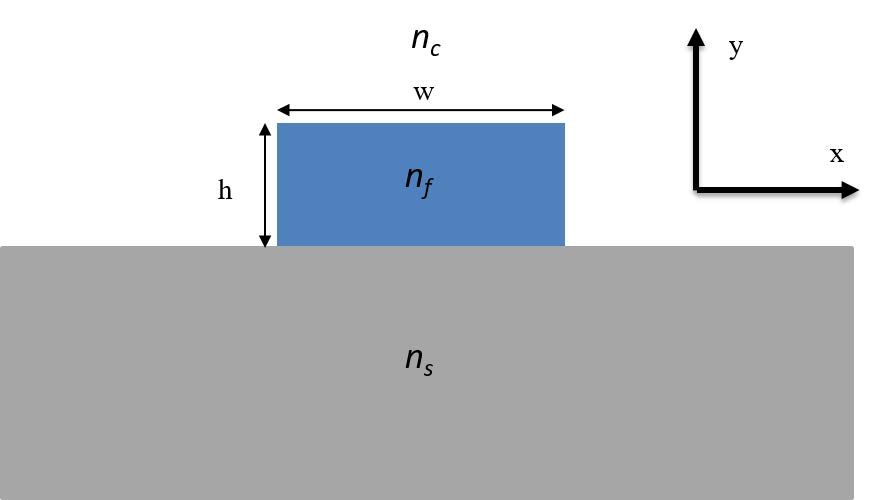
\includegraphics[width=.5\columnwidth]{A-2.jpg}
    \end{figure}
\end{prob}
\begin{sol}
    
\end{sol}
\end{document}